\documentclass{article}
\usepackage{graphicx}

\title{Estimation}
\author{Owen Xuan}

\begin{document}

\maketitle
Approximately how much does a train weigh? What’s the total late fees owed for the fall semester of OTIS? What’s an estimate for $3\sqrt{27.5}$? In each question, it’s near impossible to confidently predict a precise answer. Instead, we use logic, prior knowledge, and perhaps tools to reason out an estimate – estimation in work. Estimation itself is fundamental to the study of math, and has notably allowed mathematicians to develop theorems that more accurately describe the world. As we’ll discover, it appears in fields of math from third-grade addition to calculus.

\begin{center}
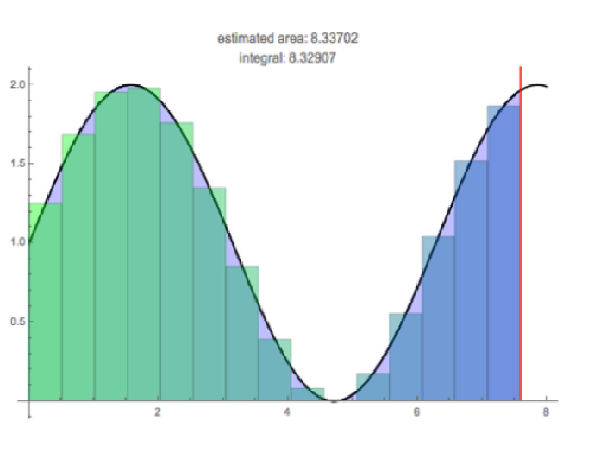
\includegraphics[scale=0.75]{images/estimate.png}
\end{center}

At the most elementary level, estimation is used in third grade classrooms in the form of rounding. Rounding lets us change numbers to become easier for humans to comprehend and thus manipulate. Even with its simplicity, rounding ubiquitously shows up in daily life: skimming the receipt for validity, say, or deciding about how many books you aim to read in the next year. However, the more interesting usages of estimation are embedded in more complex areas of math. 

Just around this time each year, many Calculus courses around the world will be teaching integration, or the study of finding the area under curves. The classical approach that will be taught is the fundamental theorem of calculus, a neat formula that produces the exact result. Yet, that very theory arose from using estimation. Specifically, after forming small rectangles as shown, the area under the curve will be approximately the total area of the rectangles; this method is called LRAM (“Left Rectangular Approximation Method”, named after Bernhard Riemann , the mathematician who is credited with discovering the method.) When you increase the number of rectangles, the estimation gets more and more precise, approaching the actual area.  

In this way, estimation precedes certainty. How else would you define integral, if not for Riemann sums? But what happens when there is no certainty? In the entire field of statistics, since data is finite and, sometimes, hard to come by,, the statistician’s job is to infer imperfect claims from the available data, rather than calculating absolute truths. As such, no statistics research article in statistics is complete without p-values and confidence rates– there simply isn’t 100 percent confidence. In addition to statistics, some numbers’ exact value cannot be determined, such as $\pi$, and e, to name a few. Moreover, as we’ll see more in depth later, most real-life situations cannot be fully described by tidy equations. Instead, they are better modeled with algorithms that accept and use uncertainty. 

\begin{center}

\includegraphics[scale=0.65]{images/esti2.png}
\end{center}

Even in cases where a clear answer exists, it’s often the case that estimating it is far more time-efficient while still producing a meaningful result. If someone aims to describe the motion of a swinging pendulum (hey, we’re now in physics!), they’ll call on differential equations (equations which involve derivatives of functions). Solving those differential equations would be arduous and annoying, but estimating them is much simpler. This can be done with Taylor series, an extremely powerful estimator tool which can also approximate polynomial functions. To use Taylor series, mathematicians take $f(x)$ on the right hand side of fig. 2, and only use the first few terms–say three. Then, after picking an arbitrary value of a for which the RHS is easily computed, they can then plug in any value for x and get an acutely accurate estimate.

\begin{align*}
    f(x) & =f(a)+\frac{f'(1)}{1!}(x-a)  \\
         & +\frac{f^{(3)}(a)}{3!}(x-a)^3+...
\end{align*} 

Now that we have some sense of a few areas of math where estimation shows up, what is the end result? Can estimation really open new doors? The answer is doubtlessly yes. Even without considering the doors it has already opened, estimation continues to lay the groundwork for mathematicians to sanity-check themselves, and quickens the pace at which they can work. Still, note that that effect is only limited to pure math. To finish, let’s return to applications: ways we use estimation in life.

If you’ve ever toyed with a synthesizer, that’s an estimator function at work, called the Fourier transform. Responses to the COVID-19 pandemic likely were informed by estimations of the potential exponential growth of infection, which at their core are just differential equations. Analysts who estimate the expected growth or fall of a stock power much of the Wall Street economy. Almost every building constructed in the US was guided by an ``Engineer's Estimate,'' wherein engineers predict the total budget needed to complete a project. Moreover, that budget estimate likely used integration (built off simple estimation techniques) to find the shape, and volume, of the building. Love your new TI-84? That calculator deconstructs difficult queries into their corresponding Taylor series, which then approximates the result.

Estimation isn’t just another small tool in a mathematician's kit– it’s more akin to their Phillips-head screwdriver.
\end{document}